% что я сделал:
% пересмотр механизма взаимодействия тасков
% реализован таск ``словарь паролей''
% изменен механизм работы с config
% механизм разбора флагов

\section{Механизм взаимодействия тасков с основной программой}

После увеличения количества тасков и спектра решамых ими задач было решено переделать механизм взаимодействия тасков с основной частью программы. Так как для некоторых тасков необходимо передавать дополнительные входные данные, было принято решение реализации более гибкого решения. Каждый таск возвращает экземпляр класса, который реализует все необходимые функции. Такой подход позволяет так же реализовать систему настройки работы при помощи входных параметров, от которой пришлось отказаться после перехода на плагиню структуру.

Данный подход был реализован и на данный момент все таски работают по описанному выше принципу. Система разбора флагов на данный момент находиться в стадии разработки. На данный момент реализованы флаги '-i' и '-o' для указания входной и выходной дирректорий, а так же флаг без аргментов '-d' для включения отладочного режима. Но данный режим поддерживают не все таски, так как не проведен полный рефакторинг кода.

Так же ввиду такого подхода пришлось усложинить механизм работы с записью config, которая выродилась в отдельный объект и передаеться в конструктор класса-таска.

\section{Механизм разбора флагов}

Идея работы данного механизма не изменилась, мы перечисляем параметры для основного приложения, после чего указываем имя таска оканчивающиеся символом ':', после чего передаем флаги для данного таска. Внутри программы же мы разбиваем строку на ``основные флаги'' которая разбирается сразу же. остальная часть разбиваеться на строки вида ``<taskname>: <flags and values>'', которая помещаеться в QMap<QString, QString>, для дальнейшей передачи в таск как часть конфига.

Разбора параметров производиться при помощи команды c++ getargs, которая сама разбирает заданную строку, основываясь на информации о том, какие флаги должны присутствовать в строке и есть ли у них аргументы.

\section{Config класс}

Структура config, содержащая три поля: inputFolder, outputFolder, OS, превратилась в отдельный класс, ввиду увиличения количества полей (например добавления QMap с описанием всех аргументов тасков и значение флага debug), так же данный класс сожержит методы по разбору входных параметров и геттеры, для доступа к значению полей класса. 

\section{TaskGetDictionary}

Часто бывает так, что пользователи создают на своих персональных компьютерах разные файлы, в которые записывают различные пароли. Появилась идея создания словаря паролей, на основании символьных последовательностей, найденных в файлах на образе. В данный момент реализован таск, который ``читает'' все текстовые файлы и создает на их основе словарь с последовательностями символов, который записываеться в SQLite базу данных. В дальнейшем планируеться расширить перечень файлов.

Алгоритм работы данного таска представлен на рисунке \ref{png:TaskGetDictionary}

\newpage
\begin{figure}[h]
 \center{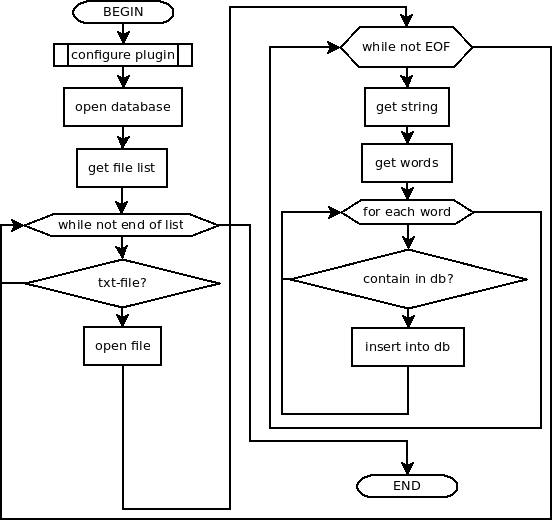
\includegraphics[width=0.7\linewidth]{getDict.png}}
 \caption{алгоритм работы таска getDictionary}
 \label{png:TaskGetDictionary}
\end{figure}
